\subsection{Hardware Optimization}
The multiply accumulate (MAC) operation is perhaps the most important and fundamental operation in signal processing and deep learning.  It has the simple form:
$$ a \leftarrow a + (b\times c) $$
This operation is fundamental in signal processing because it easily describes feedback.  However it is even more important in general because it is the building block of matrix multiplication, which can be used to describe any finite linear transformation.  Two of the most computationally intense operations in deep learning for signal analysis are filtering (convolutional layer) and matrix multiplication (fully connected layer).  Since both operations are linear, one may think of a convolutional layer as a special case of a fully connected layer but having a special structure which makes its computation faster.

There are two primary architectures for high performance MAC computation: temproal and spatial. Temporal architectures use a central controller to aggregate the data of many arithmetic logic units (ALUs).  Spatial architectures allow direct communication between many ALUs in what is called ``dataflow processing.'' ~\cite{DBLP:journals/corr/SzeCYE17} 

\begin{figure}[H]
  \centering
  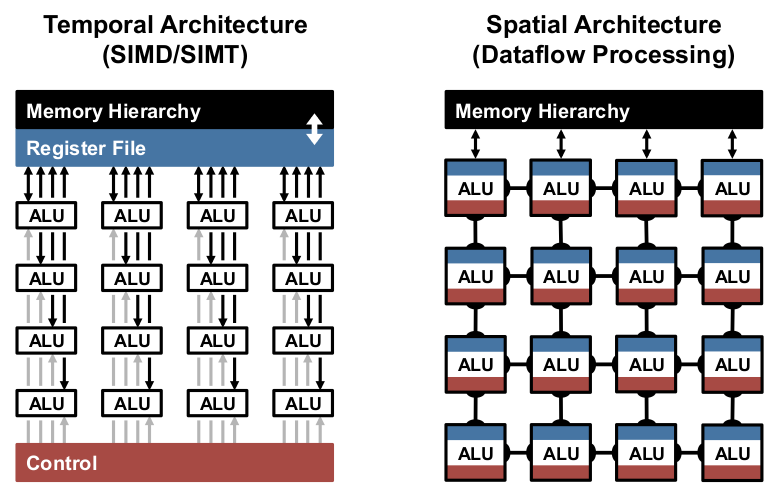
\includegraphics[width=10cm]{temporal_vs_spatial.png}
  \caption{Temporal and Spatial architectures  ~\cite{DBLP:journals/corr/SzeCYE17}}
\end{figure} 

\subsection{Operation Optimization}
\subsubsection{Theoretical Convolution}
A standard (finite) circular convolution can be computed using the ``flip and slide'' method [FF] with exactly $N_s N_f$ MACs where $N_s$ is the number of samples in the signal and $N_f$ is the number of filter coefficients.  However, it may be possible to do better.
The well known convolution theorem states that ``Convolution in the time (or spatial) domain is Hadamard (elementwise) multiplication in the frequency (temporal or spatial) domain.''  That is,
$$ x[n]\circledast y[n] = z[n] \implies X[k] \odot Y[k] = Z[k]$$
So we may calculate
$$ z[n] = \mathcal{F}^{-1}(\mathcal{F}(x[n]) \odot \mathcal{F}(y[n]))$$
It has been show that the lower bound on the number of multiplications for the fast fourier transform (for inputs of length $2^m$) is $ 4N - 2\log_2^2(N) - 2\log_2N - 4$, which has $O(N)$ complexity.  And in fact, there are known algorithms ~\cite{Winograd} which achieve this lower bound, but they use too many additions to be practical on modern processors. ~\cite{Duhamel:1990:FFT:78772.78773}  Practical algorithms such as the split-radix FFT achieve $4N\log_2{N} - 6N + 8$ real additions and multiplications, which is $O(N\log(N))$ complexity. ~\cite{Yavne:1968:EMC:1476589.1476610}  Additionally, when dealing with purely real data, there are algorithms which are capable of roughly halving the number of operations. ~\cite{Bergland:1968:NAF:364096.364118} Since our goal is to classify modulation using complex I-Q samples, it is unclear whether this optimization will be helpful, though previous work has suggested that complex neural networks offer only marginal imporvement. ~\cite{DBLP:journals/corr/TrabelsiBSSSMRB17}

It is clear that direct convolution computation has a complexity of $O(N_sN_f)$ while the Fourier transform method has a complexity of $O(N_s\log N_s)$, assuming that $N_f \leq N_s$ and we don't take advantage of the relative sparsity of the filter.  It is not immediately clear which of these is more practical.  If $N_s \rightarrow \infty$ as $N_f$ remains constant, the direct method is better.  If $N_s \rightarrow \infty$ and $N_f \rightarrow \infty$, the Fourier transform method is better.  We are also not accounting for the differing complexities and the fact that specialized hardware may exist for either.  Therefore experiment and deeper analysis will be necessary to determine which method is more suited to our application.

\subsubsection{Practical Convolution}
Many popular algorithms for fast convolution or fast Fourier Transformation run very well on processors and GPUs, but are not necessarily optimal for usage on FPGA or for real time calculation.  MIT Lincoln Laboratory has developed a systolic (spatial) FFT architecture which is designed specifically for real time operation on FPGAs and ASICs. ~\cite{Jackson}

One major practical consideration is that during inference of neural nets, the filter coefficients do not change, and the Fourier Transform of the input signal need only be generated once, no mater how many filters are used.  When performing convolution directly in the time domain, there are several strategies for minimizing memory access (which as it turns out, is the primary bottle neck). ~\cite{DBLP:journals/corr/ChetlurWVCTCS14} The primary strategies are similar to caching - the input signal or filter coefficients are stored locally (in static RAM) and reused in computations.  The downside to this is of course increased hardware for storing values statically, and the increased complexity introduced.  A descriptive diagram is shown in Figure \ref{reuse}

\begin{figure}[H]
  \centering
  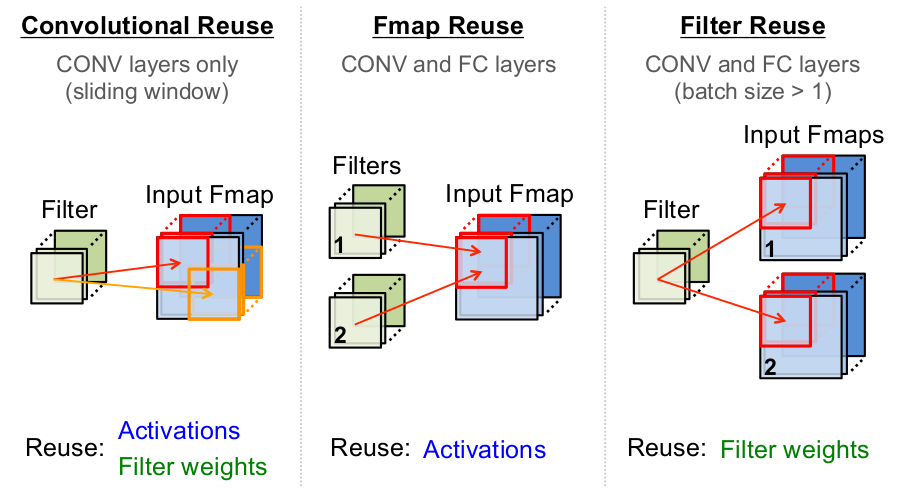
\includegraphics[width=10cm]{reuse.png}
  \label{reuse}
  \caption{Types of reuse in time domain convolution (note that activations are just the signals to be filtered) ~\cite{DBLP:journals/corr/SzeCYE17}}
\end{figure} 

\subsubsection{Theoretical Matrix Multiplication}
Fast matrix multiplication is very important in many numerical computation problems, and thus is well studied.  Two well known methods for fast matrix multiplication are Strassen's algorithm and the Coppersmith-Winograd algorithm which have complexities $O(n^{2.807})$ and $O(n^{2.376})$ respectively.  Unfortunately, the Coppersmith-Winograd algorithm is ``wildly impractical for any conceivable applications.'' ~\cite{Coppersmith:1987:MMV:28395.28396}.  Strassen's algorithm encounters similar drawbacks, it is associated with ``reduced numerical stability, increased storage requirements, and specialized processing''. ~\cite{DBLP:journals/corr/SzeCYE17}

\subsubsection{Practical Matrix Multiplication}
In practice on GPUs, no single matrix multiplication algorithm is used for every case.  Different algorithms are used depending on the shape and size and shape of the matrix. ~\cite{DBLP:journals/corr/ChetlurWVCTCS14}.  In a fully connected layer, it is almost always the case that the signal, whether it be audio, image, or video, is ``unrolled'' into a 1-D vector which is then multiplied on the left by a matrix.  Thus, in designing specialized hardware for a neural network, it may not necessarily be important that multiplication of two matrices is fast, but that multiplying a matrix and a vector is fast.  In this case there is no obvious opportunity for weight reuse since every weight in the matrix is used exactly once per vector multiplication.  However, one may think of a matrix multiplying a vector as a series of inner products between the vector and a given row of the matrix.  In this case, replicating the entire vector once for each row of the matrix may be desireable - though this comes with an $O(N_s N_r)$ (where $N_r$ is the number of rows in the matrix) static memory complexity which may be prohibitively large in some cases.
